\documentclass{article}
\usepackage{amsmath, amssymb}
\usepackage{array}
\usepackage[utf8]{inputenc}
\usepackage{graphicx}
\usepackage{subcaption}
\usepackage{enumitem}

\usepackage[super,square]{natbib} 

\usepackage[margin=1in]{geometry}
\usepackage{floatrow}
\floatsetup[table]{capposition=top}

\linespread{1.2}
\title{Assignment 3, Parallel Computing}
\author{Jinghua Feng, 661-545-981, fengj3@rpi.edu}


\begin{document}
\maketitle
\section{Setup Blue Gene/Q (BG/Q)}
In CCI Blue Gene/Q system, the main steps of obtaining execution contains three steps: compile, srun, and sbatch.
\begin{enumerate}[label=(\alph*)]
	\item compile: one should load "xl" before using compiler "mpicc" in BG/Q. See below commands for compiling code "p2p.c" to executable file "p2p.xl".
	\begin{verbatim}
	 module load xl
	 mpicc -g p2p.c -lm -o p2p.xl
	\end{verbatim}
	\item srun: The bash script file "run\_p2p.sh" for srun is shown below, in which \# of ranks (as every node contains 64 ranks) is passed to the filename of output.
	\begin{verbatim}
	#!/bin/sh
	fname="output_"
	let "rank = 64 * $1"
	srun --ntasks-per-node=64 --overcommit -o "$fname$rank" \
	/gpfs/u/home/PCP8/PCP8fngj/barn/p2p.xl
	\end{verbatim}
	\item sbatch: another bash script is applied to execute "srun" iteratively as we have to run with different MPI ranks. "n" is the number of nodes. Thus $n=1$ corresponds to 64 ranks, and $n=128$ corresponds to 8192 ranks.
	\begin{verbatim}
	#!/bin/sh
	n=1
	while [ "$n" -le 128 ]
	do
	if [ "$n" -lt 64 ]; then
	    sbatch --partition debug --nodes "$n" --time 1 ./run_p2p.sh "$n"
	elif [ "$n" -eq 64 ]; then
	    sbatch --partition small --nodes 64 --time 1 ./run_p2p.sh 64
	else
	    sbatch --partition medium --nodes 128 --time 1 ./run_p2p.sh 128
	fi
	n=$(( n*2 ))
	done
	
	\end{verbatim}
\end{enumerate}


\section{Collective - execution at different ranks}
The execution versus number of ranks based on collective approach is shown in Table 1 and Figure 1 below, which indicates that execution time is decreasing with the increase rank number. Moreover, the execution time is reduced to its half when MPI ranks double every time. This is reasonable as when MPI ranks is doubled, the size of local array to be summed in each rank is reduced by half.
\begin{table}[!htb]\centering
	\begin{tabular}{|c|c|c|c|c|c|c|c|c|}
		\hline
		Rank & 64 & 128 & 256 & 512 & 1024 & 2048 & 4096 & 8912\\
		\hline
		Execution/s & 0.743647 & 0.372150 & 0.188339 & 0.094208 & 0.047130 & 0.023601 & 0.011818 & 0.005934 \\
		\hline
	\end{tabular}
\caption{ Execution time of collective method at differnet MPI ranks}
\end{table}


\begin{figure}[!htb]
	\centering
	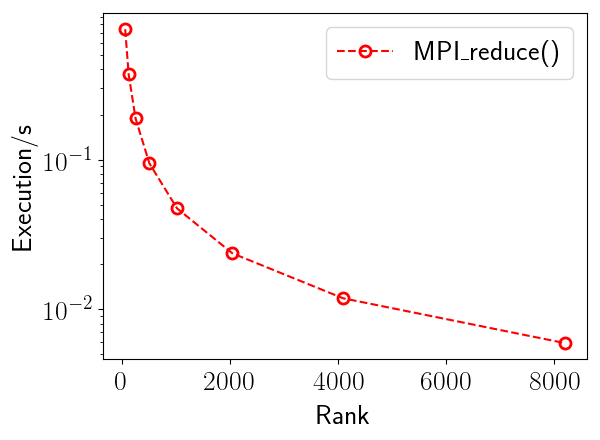
\includegraphics[scale=0.5]{../output/collective.png}
	\caption{ Execution time of collective method at differnet MPI ranks}
\end{figure}


\section{Point2Point - execution at different ranks}
The execution versus number of ranks based on point2point approach is shown in Figure 2 below, which has almost the same trend with collective method.

\begin{table}[!htb]\centering
	\begin{tabular}{|c|c|c|c|c|c|c|c|c|}
		\hline
		Rank & 64 & 128 & 256 & 512 & 1024 & 2048 & 4096 & 8912\\
		\hline
		Execution/s & 0.744446 & 0.405087 & 0.211960 & 0.099459 & 0.051483 & 0.024759 & 0.012387 & 0.005763 \\
		\hline
	\end{tabular}
	\caption{ Execution time of P2P method at differnet MPI ranks}
\end{table}

\begin{figure}[!htb]
	\centering   
	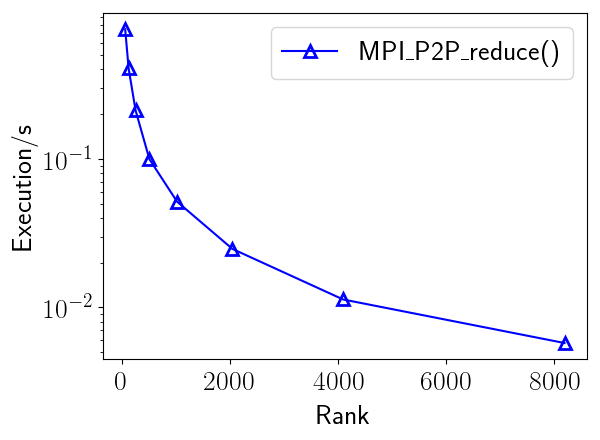
\includegraphics[scale=0.5]{../output/p2p.png}
	\caption{ Execution time of Point2Point at differnet MPI ranks}
\end{figure}


\newpage
\section{Compare collective and P2P}
By comparing above Table 1 and 2, we can easily find, for most ranks, P2P manually developed is slightly slower than collective communication MPI\_reduce embedded in MPI. Based on the explanation in Pacheco's textbook\cite{Pacheco}, collective  MPI\_reduce applies similar "binary tree structure" with Point2Point implementation in our assignment. Thus both methods has the property that sum operation is done concurrently by different processes, improving the operation efficiency a lot. The same scheme applied by these two implementations leads to their close executions. However, as the developer of MPI implementation knows better about the hardware and system software, it is not surprised that MPI\_reduce deals with implementation details better, and thus performs better.\\\\
Another observation is collective approach has lower variance of execution time. For instance, by repeating the case of 16 nodes (1024 ranks) 10 times, we obtain the execution results as below Table 3 shows. It indicates that Point2Point method has relatively higher variance. Thus collective MPI\_reduce is a more stable approach, which may also benefit from the better optimization of embedded MPI routines.
\begin{table}[!htb]\centering
	\begin{tabular}{|c|c|c|}
		\hline
		& Collective & Point2Point \\
		\hline
		 1 & 0.009262  &  0.009630\\
		 \hline
		 2 & 0.009253  &  0.009633\\
		 \hline
		 3 & 0.009257  &  0.009639\\
		 \hline
		 4 & 0.009262  &  0.009638\\
		 \hline
		 5 & 0.009261  &  0.009634\\
		 \hline
		 6 & 0.009261  &  0.009629\\
		 \hline
		 7 & 0.009254  &  0.009635\\
		 \hline
		 8 & 0.009262  &  0.009639\\
		 \hline
		 9 & 0.009260  &  0.009635\\
		 \hline
		 10 & 0.009258  &  0.009634\\
		\hline
		Variance & \textbf{1.020e-11}  &  \textbf{1.064e-11}\\
		\hline
	\end{tabular}
	\caption{ Execution time of P2P method at differnet MPI ranks}
\end{table}

\newpage
\begin{thebibliography}{}
	\bibitem{Pacheco}
	Pacheco, Peter. An introduction to parallel programming. Elsevier, 2011, pp. 102-106.
\end{thebibliography}
\end{document}
